\section{Durchführung}
    \subsection{Vorversuche Gruppe B, LM1}
        Bevor mit dem Hauptversuch begonnen werden kann, müssen diverse Vorversuche durchgeführt werden, um die Versuchsparameter zu optimieren.
        \subsubsection{Aufnahme der Kennlinie von Photomultiplier 3 (PM3)}
            Als erstes soll nach Aufgabenstellung die Kennlinie des PM3 aufgenommen werden. Dafür muss zunächst die Messtechnik angeschlossen werden. In diesem Versuch wurde das Koinzidenzsignal (1·2·3) auf den Counter 1 und das einfache Signal 3 auf den Counter mit der Nummer 2 gelegt.\\
            Danach stellt man die Hochspannungen für die Multiplier 1 und 2 ($U_{1,HV}$ und $U_{2,HV}$) auf jeweils etwa $\unit[2400]{V}$ ein. Danach wird die Hochspannung für Photomultiplier 3 auf etwa $2100\unit{V}$ geregelt. Diese Gruppe erreichte für PM1 $U_{1,HV} = 2403\unit{V}$, für $U_{2,HV} = 2401\unit{V}$ und für $U_{3,HV} = 2099\unit{V}$. 
            Nun erfolgt die Evaluierung der Messdauer. Dafür muss zunächst über den relativen Fehler ermittelt werden, wie viele Counts gemessen werden sollen. 
            $$ \frac{\Delta N}{N} = N^{-\frac{1}{2}} \leq 3\unit{\%}$$
            Da die Counts poisson-verteilt sind, erhält man für $\Delta N = \sqrt{N}$. Die Zahl der zu messenden Ereignisse (Counts) ergibt sich über diese Rechnung zu 1112. Nun wählt man im Messprogramm die Option ab, die Messung nach einer bestimmten Zeit anzuhalten und misst solange, bis Counter 1 ungefähr den errechneten Wert erreicht, wobei zu beachten ist, dass der gemessene Wert größer ist, um den relativen Fehler unterhalb der $3\unit{\%}$ zu halten. Diese Gruppe hat für einen Counter-Wert von 1122 eine Messdauer $t_{Mess} = 117\unit{s}$ gemessen. Diese Zeit wird für die Aufnahme der Kennlinie benötigt.
            Für die Aufnahme der Kennlinie des PM3 wird die Spannung $U_{3,HV}$ in $50\unit{V}$-Schritten von $1800\unit{V}$ bis $2400\unit{V}$ variiert. Die Stufen werden $t_{Mess}$ lange gemessen. Die Messdaten können in Tablle \ref{ente} nachgeschlagen werden. 
            \begin{figure}
                \centering
                \begin{tabular}{c|c|c}[htbp]
                    $U_{3,HV} \unit{V}$ & N(Signal 1·2·3) & N(Signal 3)  \\ 
                    \hline  1800 &  172 &   452\\
                    1850 &  290 &   804\\
                    1900 &  464 &  1412\\
                    1950 &  637 &  2231\\
                    2000 &  899 &  3319\\
                    2050 &  984 &  5218\\
                    2100 & 1137 &  7587\\
                    2150 & 1300 & 10836\\
                    2200 & 1294 & 14539\\
                    2250 & 1350 & 19928\\
                    2300 & 1360 & 26873\\
                    2350 & 1466 & 38098\\
                    2400 & 1415 & 53476\\
                \end{tabular} 
                \caption{Messdaten für die Aufnahme der Kennlinien}
                \label{ente}
            \end{figure}
            \begin{figure}[htbp]
                \subfigure[Kennlinie des PM3 mit Signal $N_{1·2·3}$\label{n123}]{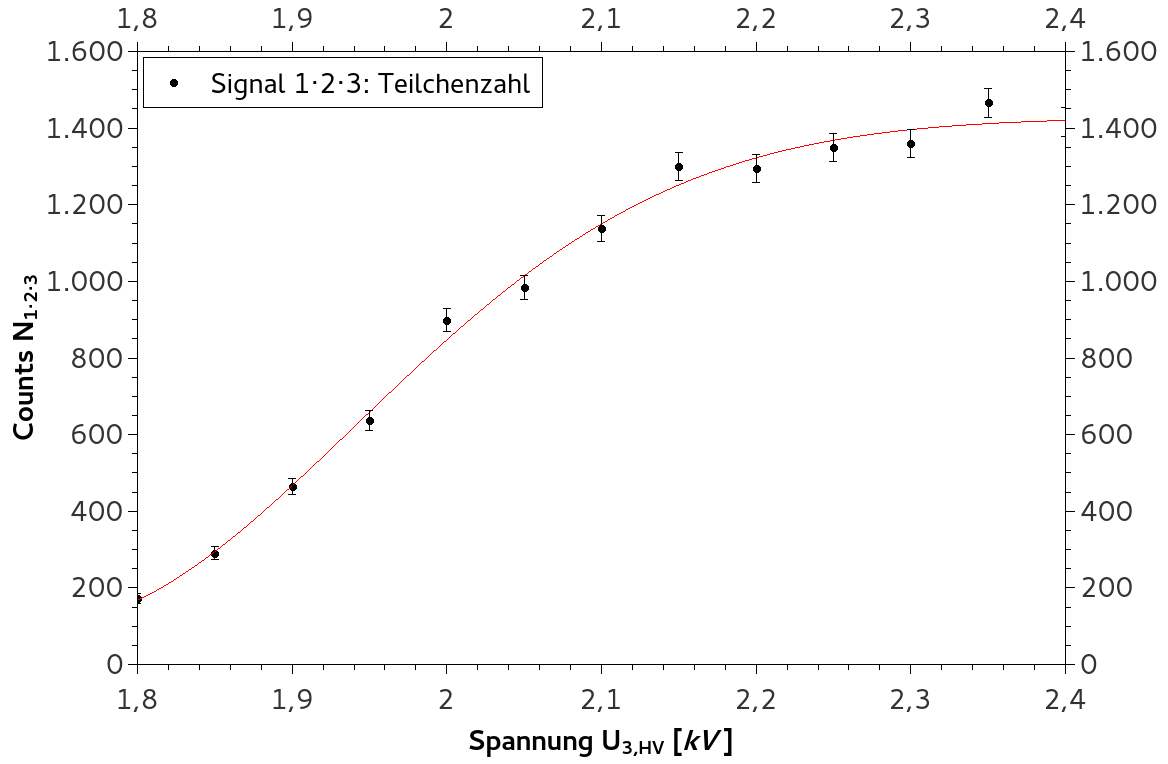
\includegraphics[scale=0.225]{pic/n123u3th}}
                \subfigure[Kennlinie des Signals $N_3$\label{n3}]{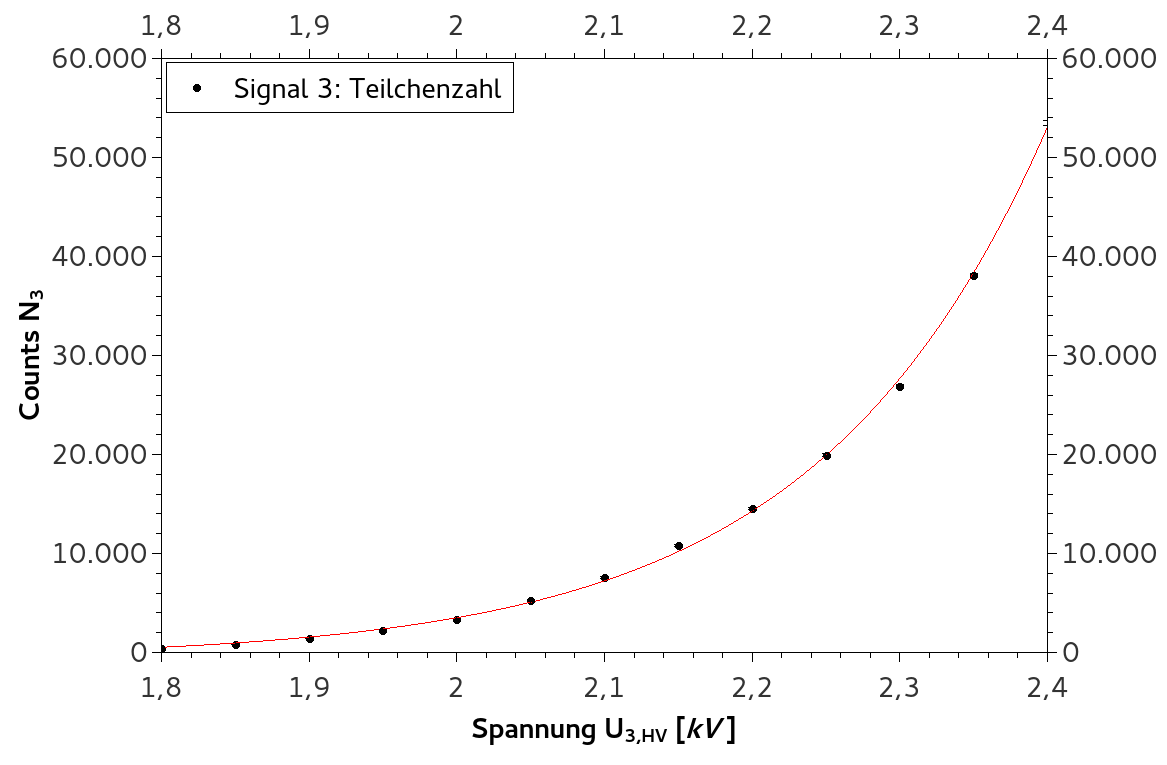
\includegraphics[scale=0.225]{pic/n3u3th}}
                \caption{Kennlinien der Hochspannung $U_{3,HV}$}
            \end{figure}
            Die Abbildungen \ref{n123} und \ref{n3} sehen sehr verschieden aus. Es ist stark auffällig, dass es sich bei \ref{n3} um ein exponentielles Wachstum handelt, während sich in \ref{n123} ein Plateau herausbildet, dessen verhalten eher einer kummulativen Verteilungsfunktion der Gauß-Kurve ähneln. 
            Die Unterschiede rühren vorallem daher, dass in \ref{n123} eine Triplezählrate vorliegt, für die Signale von allen Photomultipliern notwendig sind, um einen Count zu zählen. Es werden nur Signale gezählt, die in das Koinzidenzzeitfenster fallen und den Detektor in einer bestimmten, oben genannten Reihenfolge durchlaufen. In \ref{n3} handelt es sich um eine Singlezählrate, die nur den Photomultiplier 3 misst, dessen Hochspannung man verändert. Es wird kein Koinzidenzzeitfenster beachtet und es werden alle ankommenden Signale, bis auf das Signalrauschen, welches durch einen Diskriminator herausgefiltert wird, gemessen. Mit den steigenden Spannungen werden aus den im PM verbauten Dynoden mehr Elektronen herausgeschlagen. Damit steigt die Vervielfachung erheblich.\\
            Aus \ref{n123} kann man die Schwellspannung $U_{3,Schwell} = 2250\unit{V}$ ablesen. Sie wird als Optimierungsparamter im Hauptversuch benötigt.
            \subsubsection{Messung von Myon-Pulsen}
            Nun sollen mithilfe eines Oszilloskops Myon-Pulse gemessen werden. Dafür legt man die drei Signale aus den Photomultipliern, sowie das Signal ($1\cdot 2 \cdot 3$) das Oszilloskop bei Hochspannung von: $$ U_{1/2,HV} = 2300;\ U_{3,HV} = 2100 $$. Die Diskriminatorschwellen liegen bei: $$ U_{1,D} = 200\unit{mV};\ U_{2,D} = 200,5\unit{mV};\ U_{3,D} = 200,6\unit{mV} $$. Nun werden je PM 50 Pulse aufgenommen. Die Ergebnisse dessen sind in Tabelle \ref{pulses} nachlesbar. Daraus kann man Minima, Maxima und Mittelwerte für den jeweiligen PM bestimmen (Abb. \ref{MWs}).
            \begin{figure}[htbp]
                \centering
                \begin{tabular}{c||c|c|c|c}
                    & PM1   & PM2   & PM3 & 1·2·3\\
                    \hline $\overline U_{n}  [\unit{V}]$  & 0,990 & 0,703 & 0,878 & 0,857\\
                    $U_{n,min} [\unit{V}]$& 0,260 & 0,260 & 0,320 & 0,280\\
                    $U_{n,max} [\unit{V}]$& 4,240 & 2,840 & 2,880 & 3,320\\ 
                \end{tabular}
                \caption{Tabelle mit Minimum, Maximum und Mittelwerten}
                \label{MWs}
            \end{figure}
            Dabei fällt auf, dass PM1 den höchsten Maximumwert aufweist, was daran liegen könnte, dass dies der oberste Detektor ist und somit alle Partikel zunächst diesen passieren müssen. 
            Mit den Daten aus \ref{pulsen} kann mithilfe einer sogenannten Landau-Verteilung das Spektrum der PM-Signale dargestellt werden. Diese Verteilung ist numerisch folgendermaßen definiert:
            \begin{equation}
            p(x) = \frac{1}{\pi} \int_{0}^{\infty} \sin(\pi t)\cdot e^{-t\ln(t)-xt} dt
            \label{allgnumlf}
            \end{equation}
            Für die Plots wurde jedoch eine Approximation verwendet, die wie folgt definiert ist, da sie sich als Fit-Funktion wesentlich besser eignet als \ref{allgnumlf}:
            \begin{eqnarray}
            p(x) = \frac{1}{\sqrt{2\pi}}e^{-\frac{1}{2}\left(x+e^{-x}\right)}\\                
            p(x) = \frac{A}{\sqrt{2\pi}}e^{-\frac{1}{2}\left(\frac{x-x_0}{\sigma}+e^{-\frac{x-x_0}{\sigma}}\right)}
            \label{qtilandaufitfunktion}
            \end{eqnarray}
            In \ref{qtilandaufitfunktion} beschreiben der Parameter $A$ die Amplitude des Peaks, $x_0$ seine Verschiebung auf der x-Achse und $\sigma$ die Breite des Peaks. 
            Die Funktion \ref{qtilandaufitfunktion} fittet Verteilungen, die asymmetrisch verlaufen, kann sich jedoch auch einer Gauß-Funktion annähern.  Hier wird sie verwendet, da sie Peaks beschreibt, die auf der einen Seite stark ansteigen und auf der anderen Seite lange brauchen, um zu fallen. 
            Für das Experiment passt die Funktion, da sie die Verteilung des Energieaustritts aus den Szintillatorschichten durch Stoßionisation oder die im Szintillator deponierte Energie beschreibt, was man in den Abbildungen \ref{pm1} bis \ref{pm3} sehen kann.
                \begin{figure}[htbp]
                    \subfigure[PM1, Binbreite:0,2\label{pm1}]{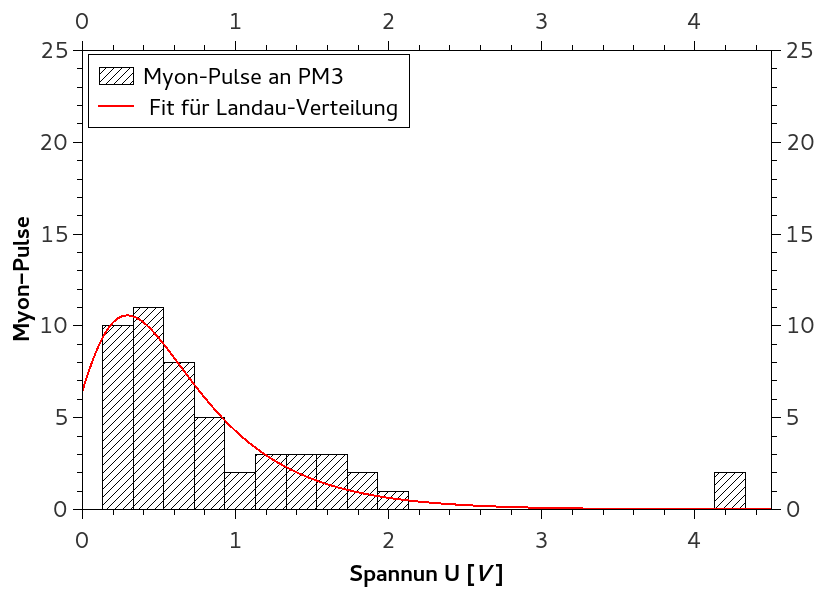
\includegraphics[scale=0.19]{pic/PM1.png}}
                    \subfigure[PM2, Binbreite:0,2\label{pm2}]{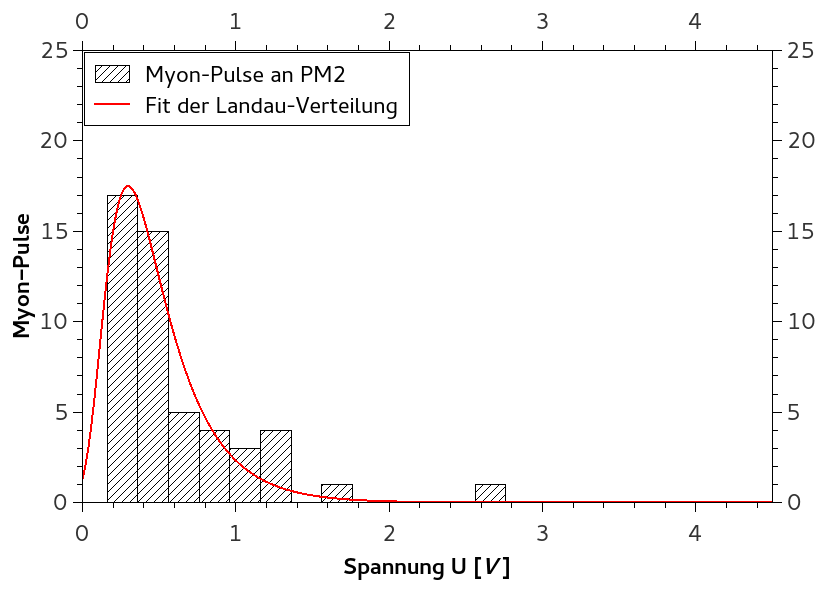
\includegraphics[scale=0.19]{pic/PM2.png}}
                    \subfigure[PM3, Binbreite:0,2\label{pm3}]{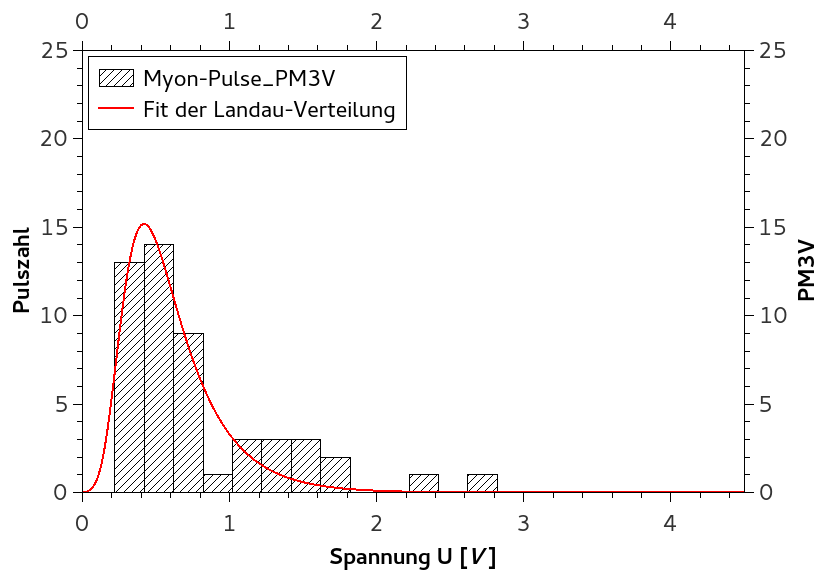
\includegraphics[scale=0.19]{pic/PM3.png}}
                    \caption{Spektren der Energieverteilung der im Detektor deponierten Energien}
                    \label{spektren}
                \end{figure}
                Das Fitten dieser Funktionen ist mit einem großen Fehler behaftet, was sich in einiger Entfernung vom Peak deutlich in allen drei Abbildungen erkennen lässt, da die dort sichtbaren Counts nicht mehr berücksichtigt werden.
                \begin{figure}[htbp]
                    \tiny\centering
                    \begin{tabular}{c|c|c}
                        Spannung $U_{PM1} [\unit{V}]$ & Spannung $U_{PM2} [\unit{V}]$ & Spannung $U_{PM3} [\unit{V}]$ \\ 
                        \hline       0,260 & 0,492 & 1,320\\
                        0,380 & 0,536 & 0,320\\
                        0,400 & 1,030 & 0,440\\
                        0,680 & 0,320 & 0,960\\
                        0,620 & 1,360 & 0,800\\
                        4,240 & 1,120 & 1,240\\
                        0,440 & 0,460 & 0,640\\
                        0,840 & 0,520 & 1,640\\
                        1,320 & 0,320 & 0,440\\
                        1,080 & 0,840 & 1,280\\
                        1,760 &	0,760 & 0,720\\
                        0,296 & 1,380 & 0,840\\
                        1,480 & 0,660 & 0,720\\
                        0,640 & 1,140 & 0,720\\
                        2,000 & 0,360 & 0,720\\
                        0,420 & 0,300 & 0,320\\
                        0,940 & 0,920 & 0,440\\
                        0,440 & 0,860 & 0,620\\
                        0,500 & 0,408 & 0,464\\
                        0,920 & 0,340 & 0,620\\
                        0,640 & 0,260 & 1,600\\
                        0,420 & 0,260 & 0,320\\
                        0,460 & 0,500 & 0,660\\
                        0,580 & 0,300 & 0,600\\
                        0,540 & 0,560 & 0,440\\
                        2,080 & 0,280 & 1,480\\
                        0,680 & 1,360 & 0,920\\
                        0,740 & 0,340 & 1,520\\
                        0,360 & 0,800 & 0,380\\
                        4,240 & 2,840 & 1,880\\
                        0,480 & 1,020 & 0,520\\
                        1,760 & 0,320 & 0,720\\
                        1,880 & 0,520 & 1,180\\
                        1,640 & 1,440 & 1,840\\
                        0,360 & 0,640 & 0,680\\
                        0,720 & 0,500 & 0,640\\
                        0,480 & 0,420 & 0,520\\
                        0,520 & 0,940 & 0,680\\
                        0,440 & 1,240 & 0,480\\
                        0,960 & 0,280 & 0,660\\
                        1,020 & 1,700 & 0,840\\
                        0,288 & 0,500 & 0,360\\
                        1,560 & 0,480 & 0,680\\
                        1,520 & 0,620 & 0,560\\
                        0,360 & 0,480 & 0,360\\
                        1,260 & 0,320 & 0,380\\
                        1,340 & 0,440 & 1,680\\
                        0,660 & 0,600 & 0,680\\
                        0,760 & 0,440 & 2,880\\
                        1,100 & 0,620 & 2,480\\
                    \end{tabular}
                    \caption{Messdaten der Myon-Pulsmessung}
                    \label{pulsen} 
                \end{figure}
                \begin{tabular}{c|c|c|c|c}
                    & A & $U_0 [\unit{kV}]$ & $\sigma$ & Bin-Breite $[\unit{kV}]$\\
                    \hline     PM1& $44\pm3$ & $0,29\pm0,08$ & $0,26,\pm0,03$& 0,2\\
                    PM2& $72\pm6$ & $0,30\pm0,05$ & $0,14,\pm0,03$& 0,2\\
                    PM3& $63\pm7$ & $0,42\pm0,03$ & $0,14,\pm0,03$& 0,2
                \end{tabular}
                \subsection{Hauptversuch}
                Für diesen Versuchsteil benötigt man die Schwellspannungen der einzelnen Photomultiplier. $$ U_{1,Schwell} = 2400\unit{V};\ U_{2,Schwell} = 2400\unit{V};\ U_{3,Schwell} = 2250\unit{V} $$. Die Schwellspannung von PM1 und PM2 wurden von Gruppe A ermittelt und an alle Gruppen weitergegeben. Sie sind durch Ablesen von den Kennlinien-Diagrammen (vgl. Abb. \ref{n123}) mit Fehlern behaftet, die das Experiment nachhaltig beeinflussen können.
                Die Diskriminatorschwellen sind auf die gleichen Werte eingstellt wie zuvor bei der Myon-Pulsmessung.
                Die Messdauer beträgt 5 Tage, das heißt $t_{Mess} = 5\cdot24\cdot60\cdot60\unit{s} = 432000\unit{s}$